%%%%%%%%%%%%%%%%%%%%%%%%%%%%%%%%%%%%%%%%%%%%%%%%%%%%%%%%%%%%%%%%%%%%
\section{Organization and Management}
\label{sec:fdsp-apa-org}

\fixme{An introduction after a major heading helps guide readers through a section. I strongly suggest including one here. Nora.}


%%%%%%%%%%%%%%%%%%%%%%%%%%%%%%%%%%%%%
\subsection{APA Consortium Organization}
\label{sec:fdsp-apa-org-consortium}

The \dword{apa} consortium comprises \num{21} institutions, of which \num{13} are in the USA, seven in the UK, and one in the Czech Republic. The consortium is organized along the main deliverables, which are the final design of the \dword{apa} and the \dword{apa} production and installation procedures. The two main centers of \dword{apa} construction are in the USA and the UK, so usually, the two leaders of each working group represent the main stakeholders (Figure~\ref{fig:apa-consortium-structure}) to ensure that common procedures and tooling are developed. 

\begin{dunefigure}[\dword{apa} Consortium organizational chart]{fig:apa-consortium-structure}
{\dword{apa} Consortium organizational chart}
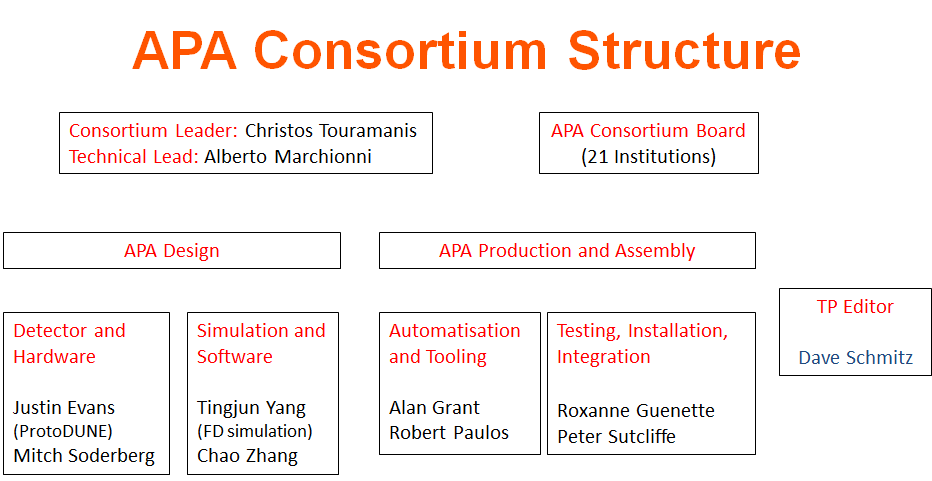
\includegraphics[width=0.95\textwidth,trim=0mm 0mm 0mm 0mm,clip]{sp-apa-consortium-structure.png}
%\includegraphics[width=0.80\textwidth]{apa-consortium-structure-new.png}  %updated org chart for consistency - Ddm
\end{dunefigure}


%%%%%%%%%%%%%%%%%%%%%%%%%%%%%%%%%%%%%%
\subsection{Planning Assumptions}
\label{sec:fdsp-apa-org-assmp}

The planning assumes eight to nine \dword{apa} assembly lines at different locations in the UK and the USA. 
We assume set up time for the factories will take about one year.
It will take approximately \num{50} shifts to construct a single \dword{apa}. Assuming a multi-shift system, we can construct the \num{150} \dwords{apa} required for one \dword{spmod} %\SI{10}{kton} module 
within about two years.

%%%%%%%%%%%%%%%%%%%%%%%%%%%%%%%%%%%%%%
\subsection{WBS and Responsibilities}
\label{sec:fdsp-apa-org-wbs}

Here, we only discuss the top-level WBS elements: (1)~design, engineering and R\&D, (2)~production setup, (3)~production, (4)~integration, and (5)~installation.

The university groups and BNL are responsible for validating  the design, while engineering and the production set up will be developed at PSL in Madison (USA) \fixme{Madison should be better identified: Madison, WI (USA)? The Daresbury Laboratory probably should have better identification as well.} and Daresbury Laboratory (UK), where the \dwords{apa} for \dword{pdsp} have been built, with contributions from university groups. \fixme{from Nora: I think what you mean here is that the university groups will contribute to developing the engineering and production set up. To make that clear, you likely will need another sentence instead of "with contributions from university groups". So "The university groups will contribute to developing..."} In addition to PSL and Daresbury Laboratory, the University of Chicago and Yale University have been identified as candidate sites for the production. The production sites will require significant help from university groups during the production process. 

In total, we expect to produce half of the \dwords{apa} in the USA and half in the UK. The steel for the frames most likely will be bought from a single vendor but will be assembled in the USA and the UK separately. We are still exploring the option to assemble the frames in house or in collaboration with industrial partners. 

Other significant components include on-\dword{apa} electronics boards. Design modifications for \dword{pdsp} are the responsibility of BNL. The boards will be produced by industry partners, but the testing will be distributed among consortium institutions. The shipping of the \dwords{apa} is the responsibility of the production factories in the USA and the UK.  The integration and installation are a joint responsibility of the Consortium, with ANL cooperating with the technical coordination group.
